\chapter{Sample chapter}
\label{cha:samplechapter}
This sample chapter serves as an illustration of frequently used elements in LaTeX such as enumerations, illustrations, tables or equations. It makes no claim to completeness and can gladly be extended. A detailed description of all commands used in LaTex can be found in the list of commands.
The samples can be copied and then adjusted.  
% Section 1 --------------------------------------------------------------
% 		Name of the section
% --------------------------------------------------------------------------
\section{Enumerations}
\label{sec:enumerations}

\subsection{Enumerations using dots}
\label{enumeration_dots}

\begin{itemize}
	\item body
	\item connecting elements
	\item coupling elements
\end{itemize}

\subsection{Enumerations using numbers}
\label{enumeration_numbers}

\begin{enumerate}
	\item body
	\item connecting elements
	\item coupling elements
\end{enumerate}

\cleardoublepage
% Section 2 --------------------------------------------------------------
% 		Name of the section
% --------------------------------------------------------------------------
\section{Illustrations}
\label{sec:illustrations}

\begin{figure}[htbp]
	\centering
		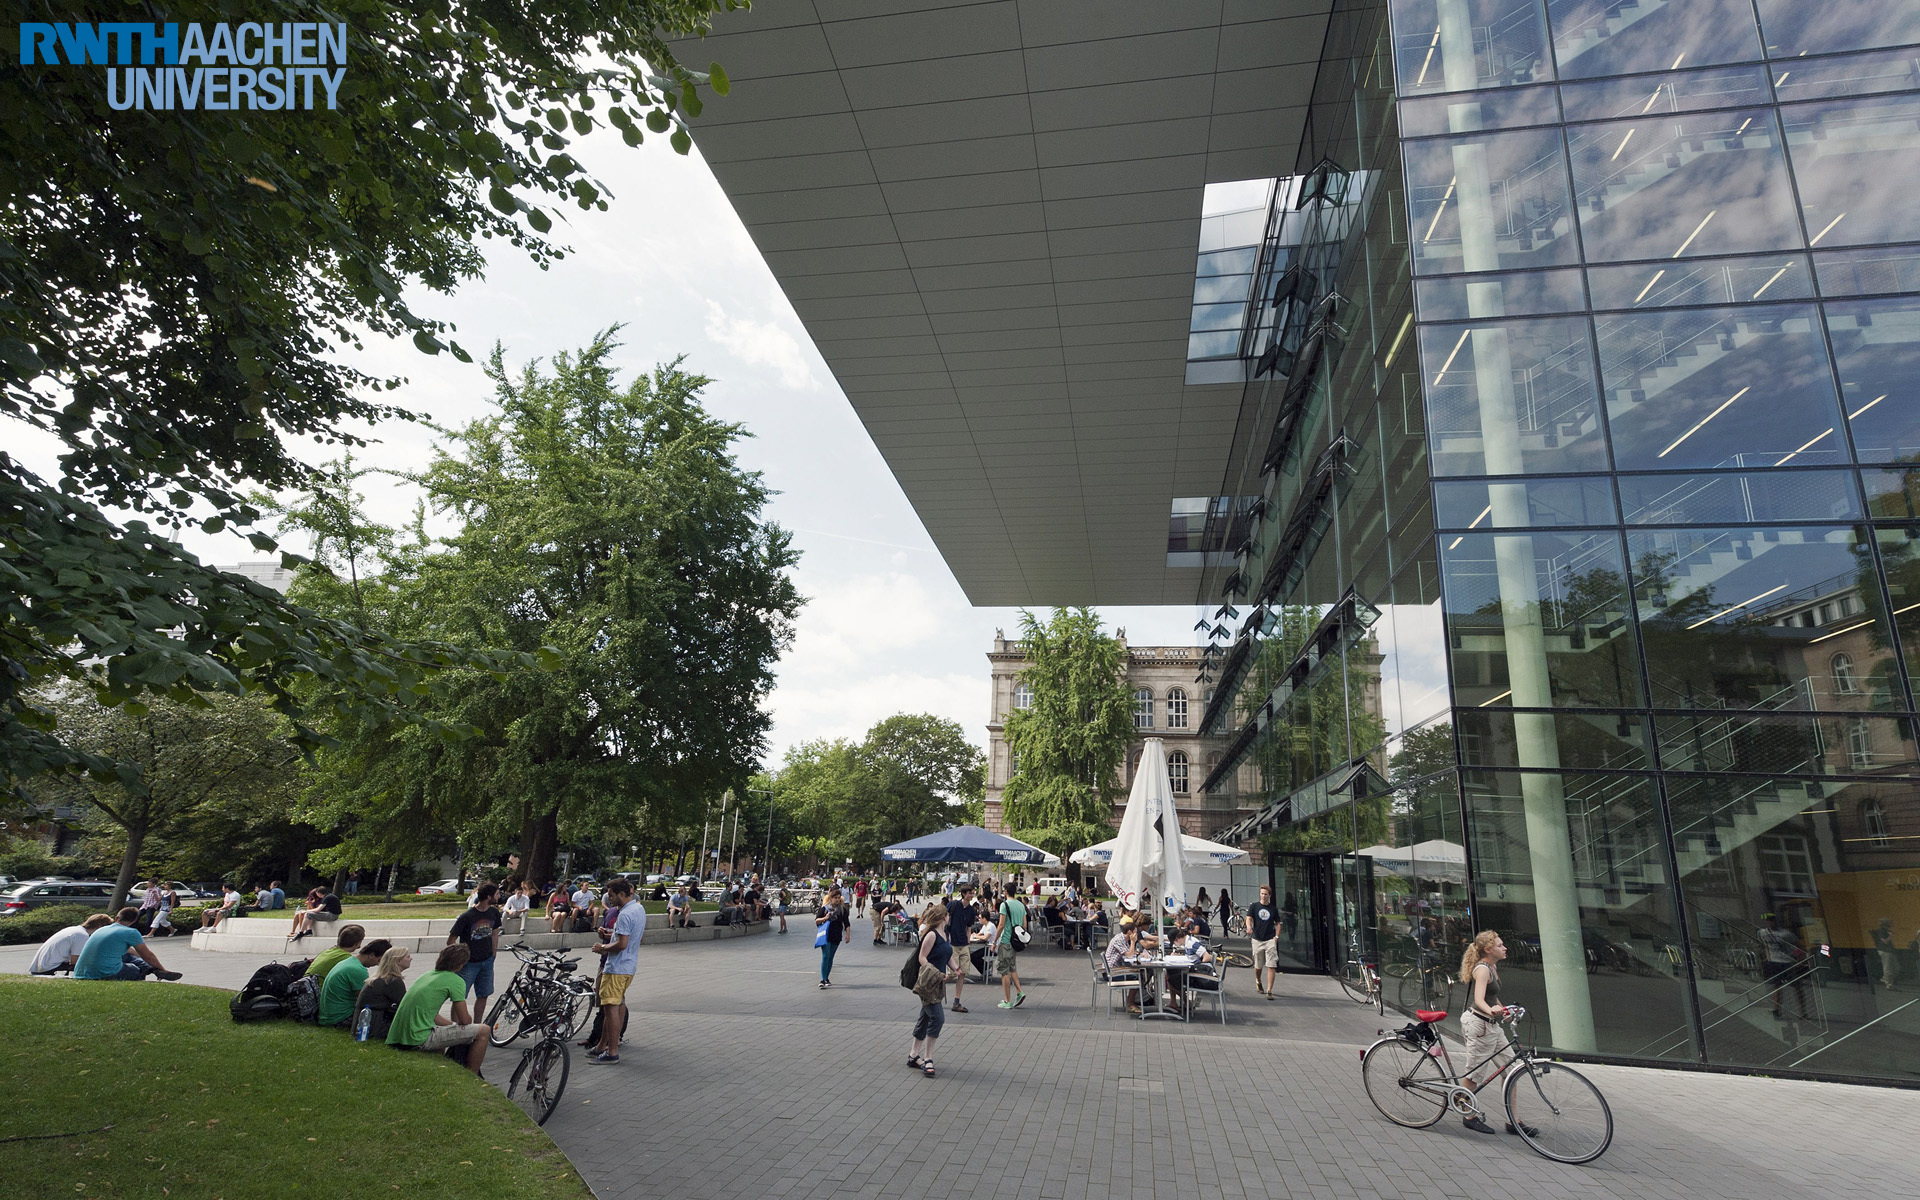
\includegraphics[width = 0.5\textwidth]{Contents/Resources/superc.jpeg}
	\caption[Image (short caption without source)]{Image (detailed caption including source, Source: \cite[1]{Sample.2012})}
	\label{fig:a_image}
\end{figure}

\begin{figure}[htbp]
	\centering
	\begin{subfigure}[t]{0.46\textwidth}
		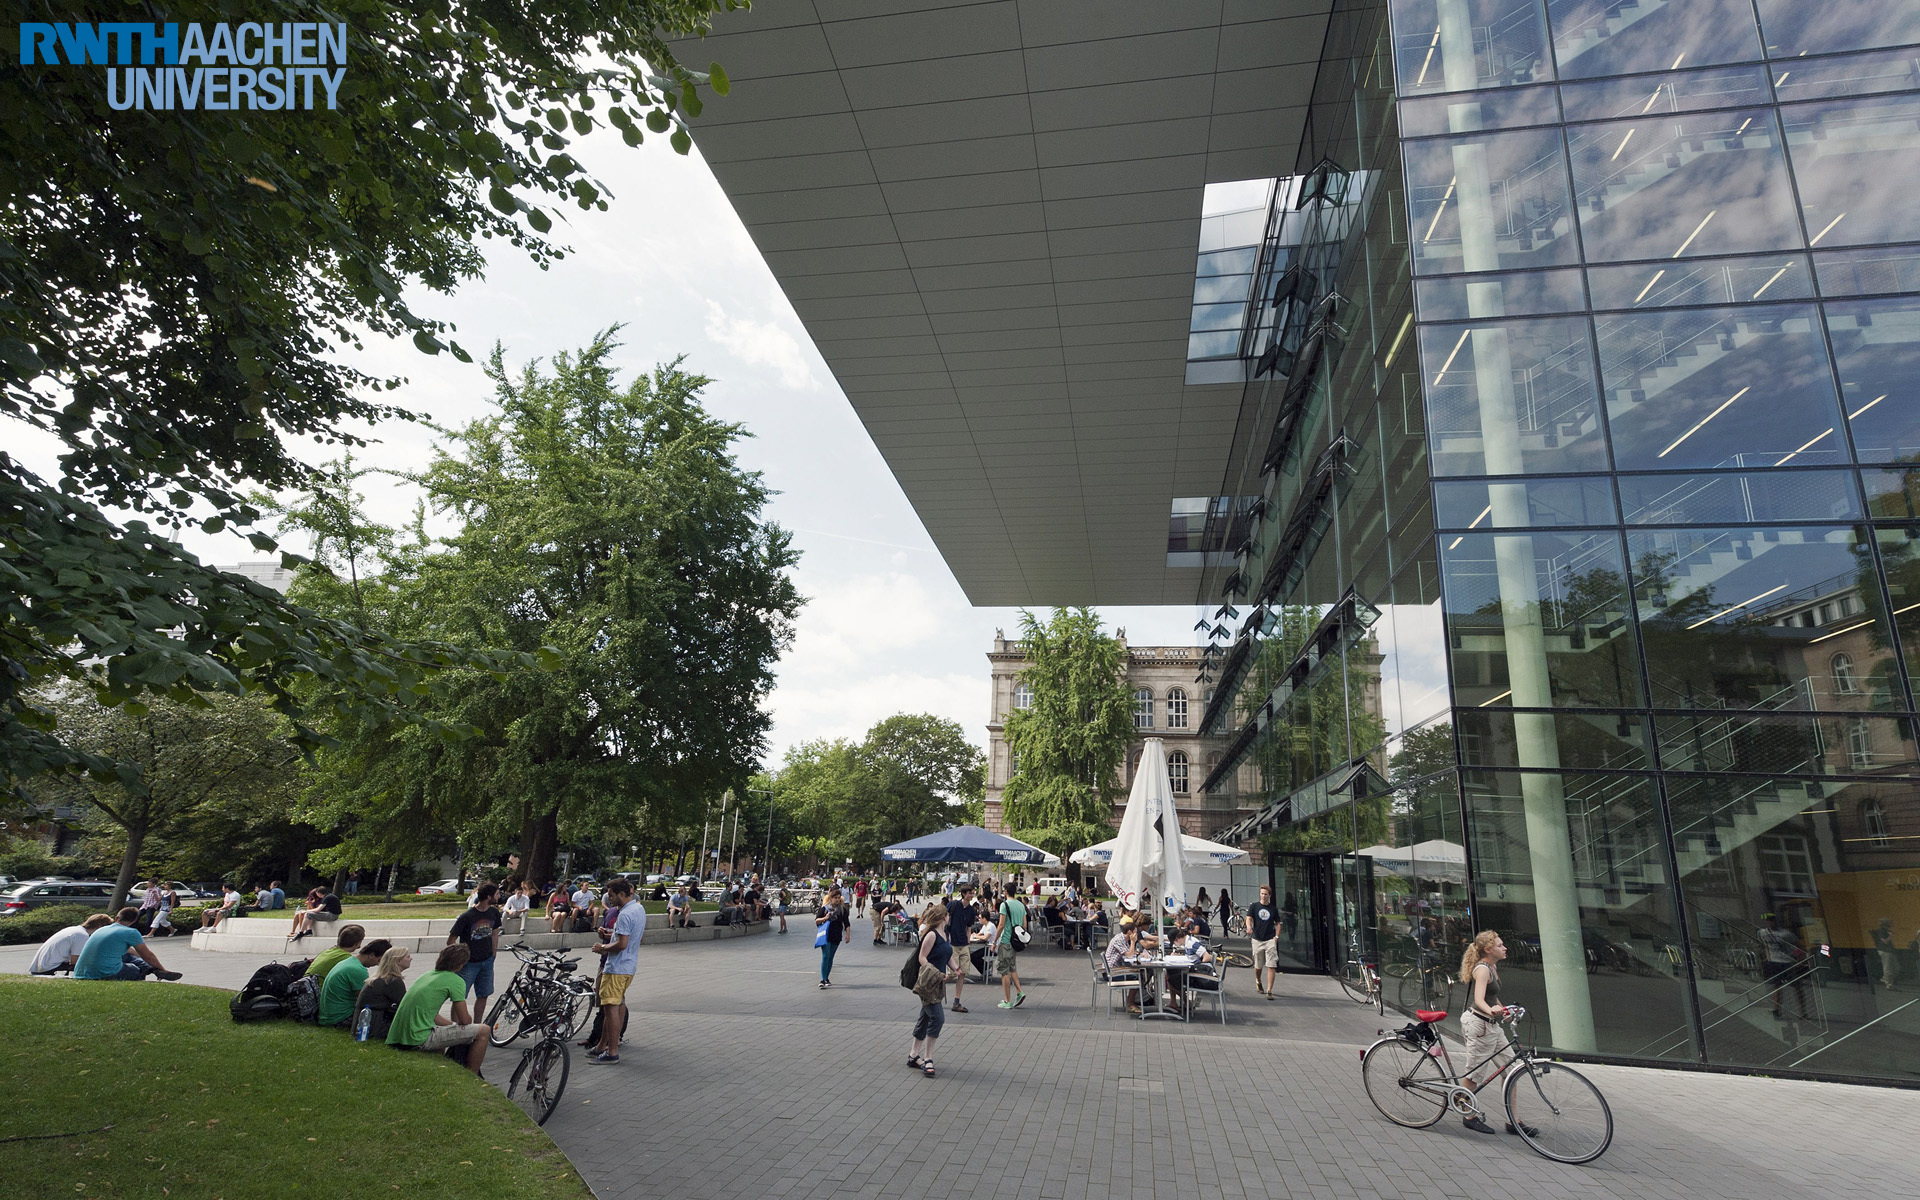
\includegraphics[width = 1\textwidth]{Contents/Resources/superc.jpeg}
		\caption{Image 1}
		\label{fig:image1}
	\end{subfigure}
	\begin{subfigure}[t]{0.46\textwidth}
		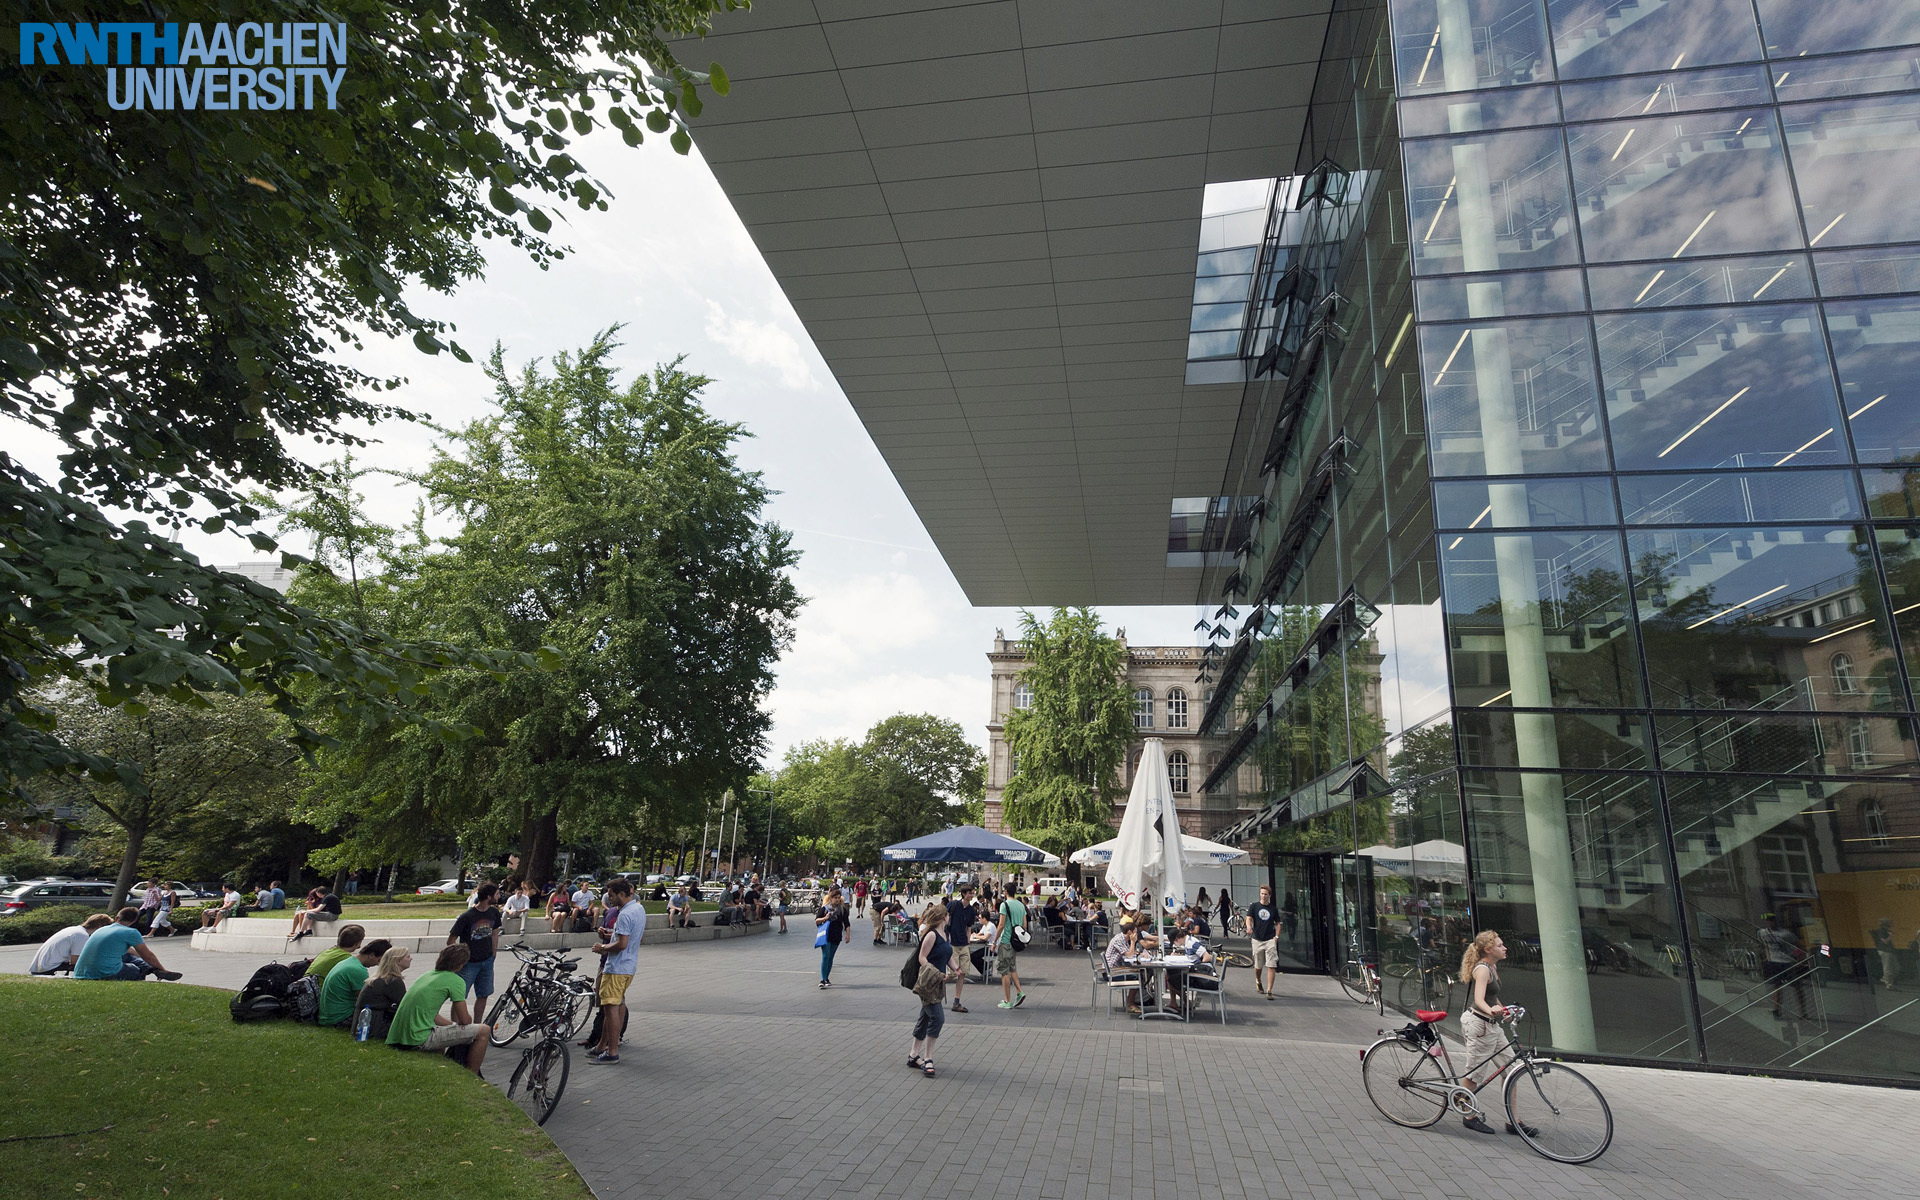
\includegraphics[width = 1\textwidth]{Contents/Resources/superc.jpeg}
		\caption{Image 2}
		\label{fig:image2}
	\end{subfigure}
	\caption[Two images]{Image 1 (a) and Image 2 (b)}
	\label{fig:multiple_images}
\end{figure}

\cleardoublepage
% Section 3 --------------------------------------------------------------
% 		Name of the section
% --------------------------------------------------------------------------
\section{Tables}
\label{sec:tables}

\begin{table}[htbp]
	\centering	
	\caption{Tables with automatic alignment}
		\begin{tabular}{lcr}
	 	\toprule
	 	l & c & r\\
	 	\midrule
		a & b & c\\[0.25em]
		aa & bb & cc\\[0.25em]
		aaa & bbb & ccc\\
		\bottomrule
	\end{tabular}	
	\label{tab:table1}
\end{table}

\begin{table}[htbp]
  \centering
  \caption{Tables aligned to seperators}
    \begin{tabular}{R{4}{3} R{4}{0}}
    \toprule
          \multicolumn{1}{c}{a} & \multicolumn{1}{c}{b}\\
    \midrule
	1,234 & 1234\\
	12,34 & 123\\
	123,4 & 12\\
	1234  & 1\\
    \bottomrule
    \end{tabular}
  \label{tab:table2}
\end{table}

\begin{table}[htbp]
	\centering	
	\caption{Table with multiple cells across various rows and columns}
		\begin{tabular}{lcr}
	 	\toprule
	 	l & c & r\\
	 	\midrule
		\multicolumn{2}{c}{ab} & c\\[0.25em]
		\multirow{2}{*}{aa} & bb & cc\\[0.25em]
		& bbb & ccc\\
		\bottomrule
	\end{tabular}	
	\label{tab:table3}
\end{table}

%\begin{table}[htbp]
%  \centering
%  \caption{multiple sub-tables}
%  \subtable[table 1]{
%    \centering  
%\begin{tabular}{lcr}
%	 	\toprule
%	 	l & c & r\\
%	 	\midrule
%		a & b & c\\[0.25em]
%		aa & bb & cc\\[0.25em]
%		aaa & bbb & ccc\\
%		\bottomrule
%	\end{tabular}	
%  }
%  \subtable[Tabelle 2]{
%    \centering  
%\begin{tabular}{lcr}
%	 	\toprule
%	 	l & c & r\\
%	 	\midrule
%		a & b & c\\[0.25em]
%		aa & bb & cc\\[0.25em]
%		aaa & bbb & ccc\\
%		\bottomrule
%	\end{tabular}	
%  }
%\label{tab:tables}
%\end{table}

\cleardoublepage
% Section 4 --------------------------------------------------------------
% 		Name of the section
% --------------------------------------------------------------------------
\section{Equations}
\label{sec:equations}

\begin{align}
	F = m a 
	\label{eqn:newton_en}
\end{align}


\section{Citation options}

Cite a source: \cite{Sample.2012}\\
Cite a source with a page reference: \cite[12-16]{Sample.2012}\\
Cite multiple Sources: \cites{Samplem.2012}{Samplef.2011}\\
Cite multiple sources with page references: \cites[12-16]{Samplem.2012}[3]{Samplef.2011}\\

